\documentclass{article}
\usepackage{graphicx} % Required for inserting images
\usepackage{amssymb}
\usepackage{amsmath}
\usepackage{amsthm}
\usepackage{hyperref}
\usepackage{float}
\usepackage{pgfplots}
\pgfplotsset{compat=1.18}

\theoremstyle{definition}
\newtheorem{example}{Example}[section]



\hypersetup{
    pdftitle={Linear Algebra I \& Mathematics Tutorial Ib - Quiz 3: Rank \& functions - Comments},
    pdfauthor={Atrajit Sarkar},
    pdfsubject={Linear Algebra I \& Mathematics Tutorial Ib, Nagoya University, Fall 2026}
}

\title{\large Linear Algebra I \& Mathematics Tutorial Ib\\
\normalsize Nagoya University, Fall 2026\\[1.2em]
\LARGE Quiz 3: Rank \& functions - Comments}
\author{ATRAJIT SARKAR\\ \small Teaching Assistant}
\date{\today}

\begin{document}

\maketitle

\tableofcontents

\pagebreak

\section{Comment 1}\label{Comment1}

If you take any any $y \in \mathbb{R}$, then $g(x_1,x_2)=y \implies x_1-3x_2=y \implies x_1=y+3x_2$

Now if you take $x_2=t \in \mathbb{R}$, then $x_1=y+3t$ and $x_2=t$ and this gives infinity may solutions for each $t\in \mathbb{R}$, for one specific $y \in \mathbb{R}$. Hence $g$ is not injective.

\section{Comment 2}\label{Comment2}
The same argument as in \hyperref[Comment1]{Comment 1}.
Because there for any $y \in \mathbb{R}$ in your codomain you get a point in your domain. So, $\operatorname{Im}(g)=\mathbb{R}$. \\
Hence, $g$ is surjective.

\textbf{Note}: Alternatively, some students gave a really nice argument. They set $x_2=0$ and $g(x_1,0)=x_1$. Now, for any $y \in \mathbb{R}$ we can take $x_1=y$ as a solution to $g(x_1,0)=y=x_1$. Hence, easily we get surjectivity. \\

The students who did this are: \textbf{[k]}

\section{Comment 3}
$f(x_1)=f(x_2)\iff  e^{2x_1}-1=e^{2x_2}-1 \iff e^{2(x_1-x_2)}=1 \iff 2(x_1-x_2)=0 \iff x_1=x_2$. Hence, $f$ is injective.

\section{Comment 4}\label{Comment4}
Below is the correct graph of $f(x)=e^{2x}-1$. Notice that the graph passes through the origin, since $f(0)=e^{0}-1=0$, and that it approaches the horizontal line $y=-1$ as $x\to-\infty$ but never touches it, because $e^{2x}>0$ for every $x\in\mathbb{R}$.

\begin{figure}[H]
    \centering
    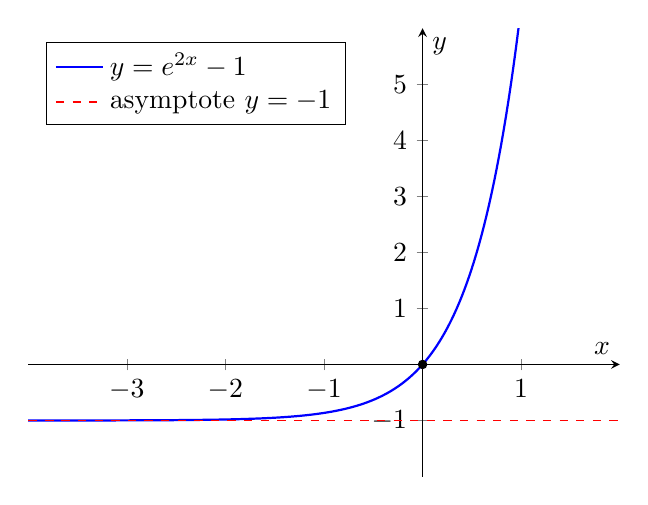
\begin{tikzpicture}
        \begin{axis}[
            axis lines=middle,
            xlabel={$x$}, ylabel={$y$},
            xmin=-4, xmax=2,
            ymin=-2, ymax=6,
            xtick={-3,-2,-1,1},
            ytick={-1,1,2,3,4,5},
            width=0.75\textwidth,
            height=0.6\textwidth,
            legend pos=north west,
            legend cell align=left,
        ]
            \addplot[domain=-4:1.0, samples=200, thick, blue] {exp(2*x)-1};
            \addlegendentry{$y=e^{2x}-1$}
            \addplot[domain=-4:2, dashed, red] {-1};
            \addlegendentry{asymptote $y=-1$}
            \addplot[only marks, mark=*, mark size=1.5pt] coordinates {(0,0)};
        \end{axis}
    \end{tikzpicture}
    \caption{The correct graph of $f(x)=e^{2x}-1$.}
\end{figure}

From the graph you can see that $\operatorname{Im}(f)=(-1,\infty)$. So, for example, $y=-2$ has no preimage: $e^{2x}-1=-2 \iff e^{2x}=-1$, which is impossible. Hence, $f:\mathbb{R}\to\mathbb{R}$ is not surjective.

\paragraph{Tip.} You can use \href{https://www.desmos.com/calculator}{desmos.com} to experiment with graphs and learn more. For example, type \texttt{y=e\^{}(2x)-1} and try changing the constants to see how the graph moves.

\section{Comment 5}\label{Comment5}
In \hyperref[Comment4]{Comment 4} we read the image of $f(x)=e^{2x}-1$ from the graph. Here is the proof that $\operatorname{Im}(f)=(-1,\infty)$. We show both inclusions.

\paragraph{$\operatorname{Im}(f)\subseteq(-1,\infty)$.} Take any $x\in\mathbb{R}$. Since $e^{2x}>0$, we get $f(x)=e^{2x}-1>-1$. So, $f(x)\in(-1,\infty)$.

\paragraph{$(-1,\infty)\subseteq\operatorname{Im}(f)$.} Take any $y>-1$. Then $y+1>0$, so $\ln(y+1)$ is defined. Put $x=\frac{1}{2}\ln(y+1)\in\mathbb{R}$. Then
\[
f(x)=e^{2\cdot\frac{1}{2}\ln(y+1)}-1=e^{\ln(y+1)}-1=(y+1)-1=y.
\]
So, every $y>-1$ has a preimage.

Hence, $\operatorname{Im}(f)=(-1,\infty)$. But the codomain is $\mathbb{R}$, and $(-1,\infty)\neq\mathbb{R}$. For example, no $y\le -1$ has a preimage. Hence, $f:\mathbb{R}\to\mathbb{R}$ is not surjective.



\end{document}
